% !TeX program = pdfLaTeX
\documentclass[12pt]{article}
\usepackage{amsmath}
\usepackage{graphicx,psfrag,epsf}
\usepackage{enumerate}
\usepackage{natbib}
\usepackage{textcomp}
\usepackage[hyphens]{url} % not crucial - just used below for the URL
\usepackage{hyperref}
\providecommand{\tightlist}{%
  \setlength{\itemsep}{0pt}\setlength{\parskip}{0pt}}

%\pdfminorversion=4
% NOTE: To produce blinded version, replace "0" with "1" below.
\newcommand{\blind}{0}

% DON'T change margins - should be 1 inch all around.
\addtolength{\oddsidemargin}{-.5in}%
\addtolength{\evensidemargin}{-.5in}%
\addtolength{\textwidth}{1in}%
\addtolength{\textheight}{1.3in}%
\addtolength{\topmargin}{-.8in}%

%% load any required packages here


\usepackage{color}
\usepackage{fancyvrb}
\newcommand{\VerbBar}{|}
\newcommand{\VERB}{\Verb[commandchars=\\\{\}]}
\DefineVerbatimEnvironment{Highlighting}{Verbatim}{commandchars=\\\{\}}
% Add ',fontsize=\small' for more characters per line
\usepackage{framed}
\definecolor{shadecolor}{RGB}{248,248,248}
\newenvironment{Shaded}{\begin{snugshade}}{\end{snugshade}}
\newcommand{\AlertTok}[1]{\textcolor[rgb]{0.94,0.16,0.16}{#1}}
\newcommand{\AnnotationTok}[1]{\textcolor[rgb]{0.56,0.35,0.01}{\textbf{\textit{#1}}}}
\newcommand{\AttributeTok}[1]{\textcolor[rgb]{0.77,0.63,0.00}{#1}}
\newcommand{\BaseNTok}[1]{\textcolor[rgb]{0.00,0.00,0.81}{#1}}
\newcommand{\BuiltInTok}[1]{#1}
\newcommand{\CharTok}[1]{\textcolor[rgb]{0.31,0.60,0.02}{#1}}
\newcommand{\CommentTok}[1]{\textcolor[rgb]{0.56,0.35,0.01}{\textit{#1}}}
\newcommand{\CommentVarTok}[1]{\textcolor[rgb]{0.56,0.35,0.01}{\textbf{\textit{#1}}}}
\newcommand{\ConstantTok}[1]{\textcolor[rgb]{0.00,0.00,0.00}{#1}}
\newcommand{\ControlFlowTok}[1]{\textcolor[rgb]{0.13,0.29,0.53}{\textbf{#1}}}
\newcommand{\DataTypeTok}[1]{\textcolor[rgb]{0.13,0.29,0.53}{#1}}
\newcommand{\DecValTok}[1]{\textcolor[rgb]{0.00,0.00,0.81}{#1}}
\newcommand{\DocumentationTok}[1]{\textcolor[rgb]{0.56,0.35,0.01}{\textbf{\textit{#1}}}}
\newcommand{\ErrorTok}[1]{\textcolor[rgb]{0.64,0.00,0.00}{\textbf{#1}}}
\newcommand{\ExtensionTok}[1]{#1}
\newcommand{\FloatTok}[1]{\textcolor[rgb]{0.00,0.00,0.81}{#1}}
\newcommand{\FunctionTok}[1]{\textcolor[rgb]{0.00,0.00,0.00}{#1}}
\newcommand{\ImportTok}[1]{#1}
\newcommand{\InformationTok}[1]{\textcolor[rgb]{0.56,0.35,0.01}{\textbf{\textit{#1}}}}
\newcommand{\KeywordTok}[1]{\textcolor[rgb]{0.13,0.29,0.53}{\textbf{#1}}}
\newcommand{\NormalTok}[1]{#1}
\newcommand{\OperatorTok}[1]{\textcolor[rgb]{0.81,0.36,0.00}{\textbf{#1}}}
\newcommand{\OtherTok}[1]{\textcolor[rgb]{0.56,0.35,0.01}{#1}}
\newcommand{\PreprocessorTok}[1]{\textcolor[rgb]{0.56,0.35,0.01}{\textit{#1}}}
\newcommand{\RegionMarkerTok}[1]{#1}
\newcommand{\SpecialCharTok}[1]{\textcolor[rgb]{0.00,0.00,0.00}{#1}}
\newcommand{\SpecialStringTok}[1]{\textcolor[rgb]{0.31,0.60,0.02}{#1}}
\newcommand{\StringTok}[1]{\textcolor[rgb]{0.31,0.60,0.02}{#1}}
\newcommand{\VariableTok}[1]{\textcolor[rgb]{0.00,0.00,0.00}{#1}}
\newcommand{\VerbatimStringTok}[1]{\textcolor[rgb]{0.31,0.60,0.02}{#1}}
\newcommand{\WarningTok}[1]{\textcolor[rgb]{0.56,0.35,0.01}{\textbf{\textit{#1}}}}

% Pandoc citation processing

\usepackage{xcolor, soul, xspace, float, subfig, lineno}

\begin{document}


\def\spacingset#1{\renewcommand{\baselinestretch}%
{#1}\small\normalsize} \spacingset{1}


%%%%%%%%%%%%%%%%%%%%%%%%%%%%%%%%%%%%%%%%%%%%%%%%%%%%%%%%%%%%%%%%%%%%%%%%%%%%%%

\if0\blind
{
  \title{\bf \texttt{forestecology} package for modeling interspecies competition
between trees}

  \author{
        Albert Y. Kim \thanks{Albert Y. Kim is Assistant Professor, Statistical \& Data Sciences,
Smith College, Northampton, MA 01063 (e-mail:
\href{mailto:akim04@smith.edu}{\nolinkurl{akim04@smith.edu}}).} \\
    Program in Statistical \& Data Sciences, Smith College\\
     and \\     David Allen \\
    Biology Department, Middlebury College\\
     and \\     Simon P. Couch \\
    Mathematics Department, Reed College\\
      }
  \maketitle
} \fi

\if1\blind
{
  \bigskip
  \bigskip
  \bigskip
  \begin{center}
    {\LARGE\bf \texttt{forestecology} package for modeling interspecies competition
between trees}
  \end{center}
  \medskip
} \fi

\bigskip
\begin{abstract}
Move abstract below here after completed.
\end{abstract}

\noindent%
{\it Keywords:} forest ecology, competition, R, Rstats, tidyverse, sf, cross-validation,
\vfill

\newpage
\spacingset{1.45} % DON'T change the spacing!

\linenumbers

\hypertarget{abstract-350-words}{%
\section{Abstract (350 words)}\label{abstract-350-words}}

\begin{enumerate}
\def\labelenumi{\arabic{enumi}.}
\tightlist
\item
  Set the context for and purpose of the work: The scientific
  question/problem and the desiderata

  \begin{itemize}
  \tightlist
  \item
    (Eventually) modularly fitting models for interspecific competition
    and assessing them using spatial crossvalidation
  \item
    Leverage ForestGEO protocols providing standardization
  \end{itemize}
\item
  Indicate the approach and the methods: Use tidyverse, simple features,
  and tidymodels packages.

  \begin{itemize}
  \tightlist
  \item
    tidyverse: as stated in tidy tools manifesto: standadized data
    structures, functional programming with pipe, designed for humans
  \item
    sf: tidyverse-friendly package that makes wrangling and visualizing
    spatial data much easier
  \item
    tidymodels: given our spatial-crossvalidation, use tidymodels
    framework is a collection of packages for modeling and machine
    learning using tidyverse principles
  \item
    Dave: hmm, I think here we might need to mention the methods we
    implement. Something like, the package provides functions to
    specific a linear, bayesian neighborhood competition model of
    growth, then fit the model, and compare competing models with
    spatiall cross validation. Or somethign like that.
  \end{itemize}
\item
  Outline the main results: We replicate from scratch the figure in
  PLOSOne paper using Big Woods data, conduct similar analysis for SCBI
  data.

  \begin{itemize}
  \tightlist
  \item
    Code would've been way more complicated in base.
  \item
    We don't have to worry about how the component functions work, only
    that sequence/converyor belt is correct and output is correct.
  \item
    Scientist is abstracted away from ugly programming details.
  \end{itemize}
\item
  Identify the conclusions and wider implications:

  \begin{itemize}
  \tightlist
  \item
    New scientific conclusions from SCBI data
  \item
    Modularly switch out our bayesian lm() functions to anything you
    want.
  \item
    this can serve as blue print for other modeling situations.
  \end{itemize}
\end{enumerate}

\hypertarget{introduction}{%
\section{Introduction}\label{introduction}}

Repeat-censused forest plots offer excellent data to test neighborhood
models of tree competition \citet{allen_permutation_2020}
\citet{canham_neighborhood_2006} \citet{uriarte_spatially_2004}. Here we
describe an R package, \texttt{forestecology}, to do that. This package
implements the methods in \citet{allen_permutation_2020}. It provides: a
convenient way to specify and fit models of tree growth based on
neighborhood competition; a spatial cross validation method to test and
compare model fits \citet{roberts_cross-validation_2017}; and an
ANOVA-like method to assess whether the competitor identity matters in
these models. The model is written to work with ForestGEO plot data
\citet{andersonteixeira_ctfs-forestgeo_2015}, but we envision that it
could easily be modified to work with data from other forest plots,
e.g.~the US Forest Service Forest Inventory and Analysis plots
\citet{smith_forest_2002}.

\hypertarget{example}{%
\section{Example}\label{example}}

We demonstrate the \texttt{forestecology} package's features on two data
sets, both based on inventory censuses of two sites from the Smithsonian
Institution's ForestGEO international network of 72 long‐term forest
dynamics research sites \citet{andersonteixeira_ctfs-forestgeo_2015}.
First, the Michigan Big Woods Forest Dynamics Plot located at the Edwin
S. George Reserve in Pinckney, MI, USA. The 23 ha plot is situated in
mature oak-hickory forest. The canopy is dominated by white oak
(\emph{Quercus alba}), northern red oak (\emph{Q. rubra}), black oak
(\emph{Q. velutina}), shagbark hickory (\emph{Carya ovata}) and pignut
hickory (\emph{C. glabra}) \citet{allen_michigan_2020}. In the example
below, we will preface any data frames from this plot in with
\texttt{bw\_}.

Second, the Smithsonian Conservation Biology Institute (SCBI) large
forest dynamics plot, located at the Smithsonian's National Zoo and
Conservation Biology Institute in Front Royal, VA, USA. The 25.6 ha (640
x 400 m) plot is located at the intersection of three of the major
physiographic provinces of the eastern US: the Blue Ridge, Ridge and
Valley, and Piedmont provinces and is adjacent to the northern end of
Shenandoah National Park. The forest type is typical mature secondary
eastern mixed deciduous forest, with a canopy dominated by tulip poplar
(\emph{Liriodendron tulipifera}), oaks (\emph{Quercus} spp.), and
hickories (\emph{Carya} spp.), and an understory composed mainly of
spicebush (\emph{Lindera benzoin}), paw-paw (\emph{Asimina triloba}),
American hornbeam (\emph{Carpinus caroliniana}), and witch hazel
(\emph{Hamamelis virginiana}) \citet{bourg_initial_2013}. In the example
below, we will preface any data frames from this plot in with
\texttt{scbi\_}.

The code that generates Figures are included in the supplementary
materials.

We load all the necessary packages.

\begin{Shaded}
\begin{Highlighting}[]
\KeywordTok{library}\NormalTok{(tidyverse)}
\KeywordTok{library}\NormalTok{(lubridate)}
\KeywordTok{library}\NormalTok{(sf)}
\KeywordTok{library}\NormalTok{(forestecology)}
\KeywordTok{library}\NormalTok{(blockCV)}
\end{Highlighting}
\end{Shaded}

\hypertarget{preprocess-census-data}{%
\subsection{Preprocess census data}\label{preprocess-census-data}}

We start by preprocessing the census data for both sites. While
ForestGEO data protocols ensure a high degree of standardization between
site, minor variations still exist
\citet{andersonteixeira_ctfs-forestgeo_2015}. While the Big Woods data
comes pre-loaded in the \texttt{forestecology} package, we load the SCBI
data as they are saved in .csv files in the SCBI-ForestGEO-Data
repository on GitHub
\citet{gonzalez-akre_scbi-forestgeoscbi-forestgeo-data_2020}. In both
cases, we load the census data as R as ``tibble'' data frames thereby
ensuring a standardized input/output format that can be used across all
\texttt{tidyverse} packages \citet{wickham_welcome_2019}.

Furthermore, we ensure that the different variables have the correct
names, types (\texttt{dbl}, \texttt{data}, \texttt{factor}).

\hypertarget{big-woods}{%
\subsubsection{Big Woods}\label{big-woods}}

We load census data from 2008 and 2014 saved in the package, then merge
species data (genus, species, linnean classification, family, etc).

\begin{Shaded}
\begin{Highlighting}[]
\NormalTok{census_}\DecValTok{2008}\NormalTok{_bw <-}\StringTok{ }\NormalTok{census_}\DecValTok{2008}\NormalTok{_bw }\OperatorTok
\StringTok{  }\KeywordTok{left_join}\NormalTok{(species_bw, }\DataTypeTok{by =} \StringTok{"sp"}\NormalTok{) }\OperatorTok
\StringTok{  }\KeywordTok{select}\NormalTok{(}\OperatorTok{-}\KeywordTok{c}\NormalTok{(genus, species, latin))}
\end{Highlighting}
\end{Shaded}

\hypertarget{scbi-data}{%
\subsubsection{SCBI}\label{scbi-data}}

We load census data from 2008 and 2014 from \texttt{.csv} files saved
from GitHub on November 20, 2020. Furthermore, we perform two additional
pre-processing steps. First, in order to speed up computation for
purposes of this example, we only consider a 9 ha subsection of the 25.6
ha of the SCBI site: \texttt{gx} from 0--300 instead of 0--400 and
\texttt{gy} from 300--600 instead of 0--640. Second, in order to
standardize comparisons between Big Woods and SCBI, we convert the units
of dbh from mm to cm. \footnote{A rule of thumb to ascertain if dbh is
  in mm or cm is to verify if the smallest non-zero and non-missing
  measurement is 1 or 10. If the former, then cm. If the later, then mm.
  This is because ForestGEO protocols state that only trees with dbh
  greater or equal to 1cm should be included in censuses. }

\begin{Shaded}
\begin{Highlighting}[]
\NormalTok{census_}\DecValTok{2013}\NormalTok{_scbi <-}\StringTok{ }\KeywordTok{read_csv}\NormalTok{(}\StringTok{"scbi.stem2.csv"}\NormalTok{) }\OperatorTok
\StringTok{  }\KeywordTok{select}\NormalTok{(treeID, stemID, sp, ExactDate, gx, gy, dbh, codes, status) }\OperatorTok
\StringTok{  }\KeywordTok{mutate}\NormalTok{(}
    \DataTypeTok{date =}\NormalTok{ ExactDate }\OperatorTok\StringTok{ }\KeywordTok{mdy}\NormalTok{(),}
    \DataTypeTok{dbh =} \KeywordTok{as.numeric}\NormalTok{(dbh)}
\NormalTok{  ) }\OperatorTok
\StringTok{  }\KeywordTok{filter}\NormalTok{(gx }\OperatorTok{<}\StringTok{ }\DecValTok{300}\NormalTok{, }\KeywordTok{between}\NormalTok{(gy, }\DecValTok{300}\NormalTok{, }\DecValTok{600}\NormalTok{)) }\OperatorTok\StringTok{ }
\StringTok{  }\KeywordTok{mutate}\NormalTok{(}\DataTypeTok{dbh =}\NormalTok{ dbh }\OperatorTok{/}\StringTok{ }\DecValTok{10}\NormalTok{)}

\NormalTok{census_}\DecValTok{2018}\NormalTok{_scbi <-}\StringTok{ }\KeywordTok{read_csv}\NormalTok{(}\StringTok{"scbi.stem3.csv"}\NormalTok{) }\OperatorTok
\StringTok{  }\KeywordTok{select}\NormalTok{(treeID, stemID, sp, ExactDate, gx, gy, dbh, codes, status) }\OperatorTok
\StringTok{  }\KeywordTok{mutate}\NormalTok{(}
    \DataTypeTok{date =}\NormalTok{ ExactDate }\OperatorTok\StringTok{ }\KeywordTok{mdy}\NormalTok{(),}
    \DataTypeTok{dbh =} \KeywordTok{as.numeric}\NormalTok{(dbh)}
\NormalTok{  ) }\OperatorTok
\StringTok{  }\KeywordTok{filter}\NormalTok{(gx }\OperatorTok{<}\StringTok{ }\DecValTok{300}\NormalTok{, }\KeywordTok{between}\NormalTok{(gy, }\DecValTok{300}\NormalTok{, }\DecValTok{600}\NormalTok{)) }\OperatorTok\StringTok{ }
\StringTok{  }\KeywordTok{mutate}\NormalTok{(}\DataTypeTok{dbh =}\NormalTok{ dbh }\OperatorTok{/}\StringTok{ }\DecValTok{10}\NormalTok{)}
\end{Highlighting}
\end{Shaded}

\hypertarget{compute-annual-growth}{%
\subsection{Compute annual growth}\label{compute-annual-growth}}

MERGE THIS SUBSECTION with previous?

For each plot we then compute average annual growth between the two
censuses using the \texttt{compute\_growth()} function. This function
takes the two census data frames as well as a character indicating which
variable in both data frames uniquely identifies each stem. This
function returns a single data frame that includes a numerical variable
\texttt{growth} reflecting the average annual dbh growth (in cm) of all
trees alive at both time points. Furthermore, variables that (in theory)
remain unchanged between censuses appear only once, such as location
variables \texttt{gx} and \texttt{gy}; as well as species-related
variables. Variables that should change between censuses are suffixed
with \texttt{1} and \texttt{2} indicating the earlier and later
censuses, such as \texttt{dbh1/dbh2} and \texttt{codes1/codes2}. Here
the resulting data frames are named with some variation of
\texttt{growth\_df}.

After computing the average annual growth for each tree, we ensure to
convert all variables denote species from type character to factors;
this is to ensure that issues of rare species being accounted for in
both training and test sets in our upcoming cross-validation step (see
Section REF)

\hypertarget{big-woods-1}{%
\subsubsection{Big Woods}\label{big-woods-1}}

In the case of Big Woods data, we first remove all trees that were
re-sprouts in the later (2014) census. Additionally, we have included
two classification of tree species: \texttt{species} and
\texttt{family}. To illustrate model comparison, we test competition
models in which individuals are grouped by species and by family.

\begin{Shaded}
\begin{Highlighting}[]
\NormalTok{growth_bw <-}
\StringTok{  }\KeywordTok{compute_growth}\NormalTok{(}
    \DataTypeTok{census_1 =}\NormalTok{ census_}\DecValTok{2008}\NormalTok{_bw }\OperatorTok\StringTok{ }
\StringTok{      }\KeywordTok{mutate}\NormalTok{(}\DataTypeTok{sp =} \KeywordTok{to_any_case}\NormalTok{(sp) }\OperatorTok\StringTok{ }\KeywordTok{factor}\NormalTok{()),}
    \DataTypeTok{census_2 =}\NormalTok{ census_}\DecValTok{2014}\NormalTok{_bw }\OperatorTok\StringTok{ }
\StringTok{      }\KeywordTok{filter}\NormalTok{(}\OperatorTok{!}\KeywordTok{str_detect}\NormalTok{(codes, }\StringTok{"R"}\NormalTok{)) }\OperatorTok\StringTok{ }
\StringTok{      }\KeywordTok{mutate}\NormalTok{(}\DataTypeTok{sp =} \KeywordTok{to_any_case}\NormalTok{(sp) }\OperatorTok\StringTok{ }\KeywordTok{factor}\NormalTok{()),}
    \DataTypeTok{id =} \StringTok{"treeID"}
\NormalTok{  )}
\end{Highlighting}
\end{Shaded}

\hypertarget{scbi}{%
\subsubsection{SCBI}\label{scbi}}

\begin{Shaded}
\begin{Highlighting}[]
\NormalTok{growth_scbi <-}
\StringTok{  }\KeywordTok{compute_growth}\NormalTok{(}
    \DataTypeTok{census_1 =}\NormalTok{ census_}\DecValTok{2013}\NormalTok{_scbi }\OperatorTok\StringTok{ }
\StringTok{      }\KeywordTok{mutate}\NormalTok{(}\DataTypeTok{sp =} \KeywordTok{to_any_case}\NormalTok{(sp) }\OperatorTok\StringTok{ }\KeywordTok{factor}\NormalTok{()),}
    \DataTypeTok{census_2 =}\NormalTok{ census_}\DecValTok{2018}\NormalTok{_scbi }\OperatorTok\StringTok{ }
\StringTok{      }\KeywordTok{filter}\NormalTok{(}\OperatorTok{!}\KeywordTok{str_detect}\NormalTok{(codes, }\StringTok{"R"}\NormalTok{)) }\OperatorTok\StringTok{ }
\StringTok{      }\KeywordTok{mutate}\NormalTok{(}\DataTypeTok{sp =} \KeywordTok{to_any_case}\NormalTok{(sp) }\OperatorTok\StringTok{ }\KeywordTok{factor}\NormalTok{()),}
    \DataTypeTok{id =} \StringTok{"stemID"}
\NormalTok{  )}
\end{Highlighting}
\end{Shaded}

\hypertarget{comparison}{%
\subsubsection{Comparison}\label{comparison}}

DAVE: I THINK THIS FIGURE IS UNNEEDED. COULD BE REMOVED FOR SPACE
REASONS. Figure \ref{fig:growth-histogram} displays histograms comparing
the distribution of average annual growth at both sites. Observe that
average annual growth appears higher at the Big Woods site.

\begin{figure}

{\centering 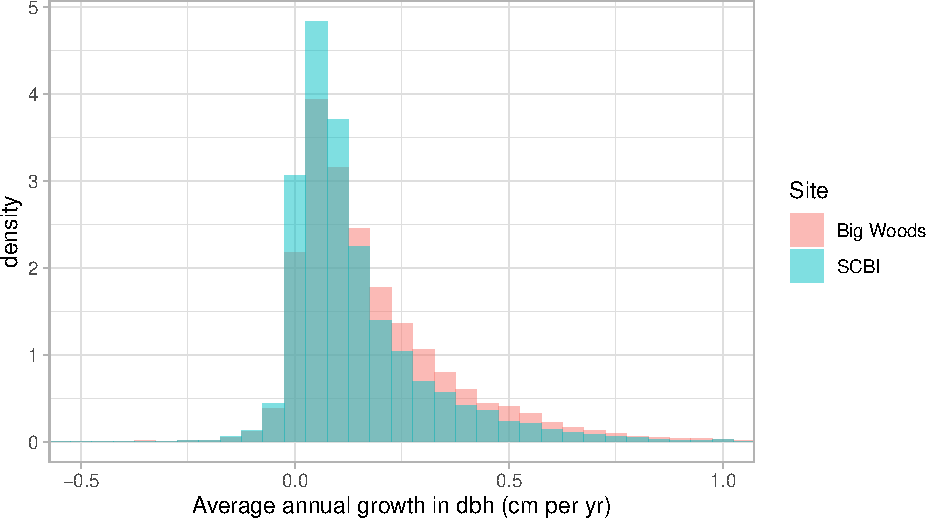
\includegraphics[width=1\linewidth]{Figures/growth-histogram-1} 

}

\caption{Distribution of average annual growth in DBH for both sites.}\label{fig:growth-histogram}
\end{figure}

\hypertarget{spatial-information}{%
\subsection{Add spatial information}\label{spatial-information}}

We now encode spatial information to the \texttt{growth\_df} data
frames. First, in order to control for study region edge effects, we add
``buffers'' to the periphery of the study region (cite Waller?). Our
model of interspecific competition relies on a spatial definition of who
the competitor trees are for focal trees of interest. Since certain
explanatory variables such as basal area are cumulative, we must ensure
that all trees being modeled are not biased to have different neighbor
structures. This is a particular concern for trees at the boundary of
study regions, which will not have the same number of neighbors as trees
in the internal part of the study region.

Second, our ultimate method for model assessment will rely on estimates
of model error as generated by cross-validation. Conventional
cross-validation schemes assign observations to folds by resampling
individual observations at random. However, underlying this scheme is an
assumption that the observations are independent. In the case of forest
census data, observations exhibit spatial autocorrelation, and thus this
dependence must be incorporated in our resampling scheme in spatial
cross-validation \citet{roberts_cross-validation_2017}
\citet{pohjankukka_estimating_2017} We will therefore associate portions
of the study region to spatial folds.

To these two ends, we define two constants, both of which are in the
same units as the \texttt{gx} and \texttt{gy} variables (most often
meters).

\begin{Shaded}
\begin{Highlighting}[]
\NormalTok{comp_dist <-}\StringTok{ }\FloatTok{7.5}
\NormalTok{cv_fold_size <-}\StringTok{ }\DecValTok{100}
\end{Highlighting}
\end{Shaded}

The first constant is \texttt{comp\_dist} which defines the maximum
distance for a tree's competitive neighborhood. Trees within this
distance of each other are assumed to compete while those farther than
this distance apart do not. Put differently, all trees within
\texttt{comp\_dist} of a focal tree will be considered its competitors
(see below). Other studies have estimated the value of
\texttt{comp\_dist}; we use an average of estimated values
\citet{canham_neighborhood_2004}, \citet{uriarte_spatially_2004},
\citet{tatsumi2013}, \citet{canham_neighborhood_2006}.

Furthermore, \texttt{comp\_dist} will define the size of all buffers
considered, which will be encoded as a binary variable \texttt{buffer}
as computed by the \texttt{add\_buffer\_variable()} function. This
function takes as input the main \texttt{growth\_df} data frame, the
\texttt{size} of the buffer which we set as \texttt{comp\_dist}, and the
boundary of the study region encoded as a simple features polygon
\citet{pebesma_simple_2018}. DESCRIBE SF PACKAGE. In the Big Woods
example below we will use a pre-loaded simple features polygon while for
the SCBI example we present example code on how to manually construct
one.

The second constant is \texttt{cv\_fold\_size} which defines the length
and width of the spatial folds (note that for now the spatial folds are
restricted be squares). We will then use this constant to associate each
observed tree to one of \(k\) folds in the respective study region. In
the Big Woods example below we will use the \texttt{blockCV} R package
that has implemented spatial cross-validation while for the SCBI we will
do this manually \citet{valavi_blockcv_2019}

\hypertarget{big-woods-2}{%
\subsubsection{Big Woods}\label{big-woods-2}}

First, we indicate which trees are part of the buffer. This necessitates
information about the study region boundary. In this case, we use a
\texttt{sf\_polygon} object \texttt{study\_region\_bw} which comes
pre-loaded in the \texttt{forestecology} packages. After loading
\texttt{study\_region\_bw}, we illustrate the results of the
\texttt{add\_buffer\_variable()} function in Figure
\ref{fig:bw-define-buffer}. Trees on the periphery denote with lighter
colors are part of the buffer and will not be considered as ``focal''
trees of interest going forward; they will only be considered as
competitor trees.

\begin{Shaded}
\begin{Highlighting}[]
\KeywordTok{data}\NormalTok{(study_region_bw)}

\NormalTok{growth_bw <-}\StringTok{ }\NormalTok{growth_bw }\OperatorTok
\StringTok{  }\KeywordTok{add_buffer_variable}\NormalTok{(}\DataTypeTok{direction =} \StringTok{"in"}\NormalTok{, }\DataTypeTok{size =}\NormalTok{ comp_dist, }\DataTypeTok{region =}\NormalTok{ study_region_bw)}

\KeywordTok{ggplot}\NormalTok{() }\OperatorTok{+}
\StringTok{  }\KeywordTok{geom_sf}\NormalTok{(}\DataTypeTok{data =}\NormalTok{ growth_bw }\OperatorTok\StringTok{ }\KeywordTok{sample_frac}\NormalTok{(}\FloatTok{0.2}\NormalTok{), }\KeywordTok{aes}\NormalTok{(}\DataTypeTok{col =}\NormalTok{ buffer), }\DataTypeTok{size =} \FloatTok{0.5}\NormalTok{)}
\end{Highlighting}
\end{Shaded}

\begin{figure}

{\centering 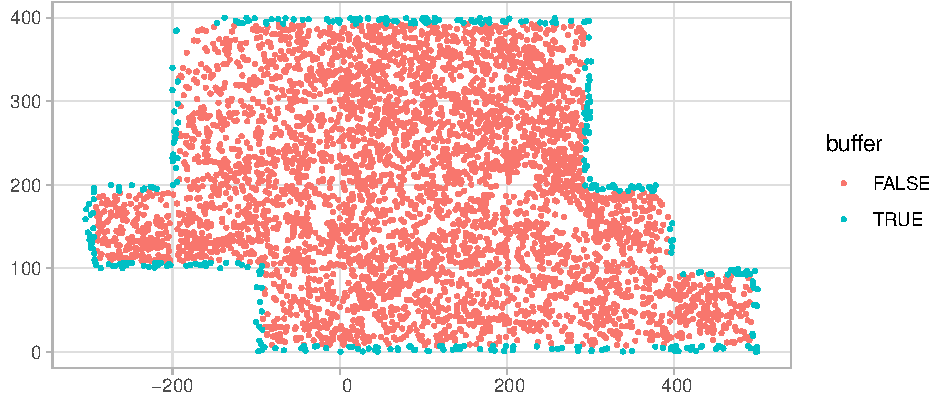
\includegraphics[width=1\linewidth]{Figures/bw-define-buffer-1} 

}

\caption{Buffer region for Big Woods study region.}\label{fig:bw-define-buffer}
\end{figure}

Second, we associate each tree to spatial cross validation folds. In
this case, we use the \texttt{spatialBlock()} function from the
\texttt{blockCV} package to define the spatial grid which

THIS IS A MESS. We use the \citet{valavi_blockcv_2019}, whose elements
will act as the folds in our leave-one-out (by ``one'' we mean ``one
grid block'') cross-validation scheme. The upshot here is we add
\texttt{foldID} to \texttt{growth\_df} which identifies which fold each
individual is in, and the creation of a \texttt{cv\_grid\_sf} object
which gives the geometry of the cross validation grid.

\begin{Shaded}
\begin{Highlighting}[]
\KeywordTok{set.seed}\NormalTok{(}\DecValTok{76}\NormalTok{)}
\NormalTok{bw_spatialBlock <-}\StringTok{ }\KeywordTok{spatialBlock}\NormalTok{(}
  \DataTypeTok{speciesData =}\NormalTok{ growth_bw, }\DataTypeTok{theRange =}\NormalTok{ cv_fold_size, }\DataTypeTok{k =} \DecValTok{28}\NormalTok{, }\DataTypeTok{xOffset =} \FloatTok{0.5}\NormalTok{, }
  \DataTypeTok{yOffset =} \DecValTok{0}\NormalTok{, }\DataTypeTok{verbose =} \OtherTok{FALSE}\NormalTok{, }\DataTypeTok{showBlocks =} \OtherTok{FALSE}
\NormalTok{)}
\end{Highlighting}
\end{Shaded}

Then add foldID to each tree

\begin{Shaded}
\begin{Highlighting}[]
\NormalTok{growth_bw <-}\StringTok{ }\NormalTok{growth_bw }\OperatorTok
\StringTok{  }\KeywordTok{mutate}\NormalTok{(}\DataTypeTok{foldID =}\NormalTok{ bw_spatialBlock}\OperatorTok{$}\NormalTok{foldID)}
\end{Highlighting}
\end{Shaded}

\begin{Shaded}
\begin{Highlighting}[]
\CommentTok{# Visualize grid. Why does fold 19 repeat?}
\KeywordTok{ggplot}\NormalTok{() }\OperatorTok{+}
\StringTok{  }\KeywordTok{geom_sf}\NormalTok{(}\DataTypeTok{data =}\NormalTok{ bw_spatialBlock}\OperatorTok{$}\NormalTok{blocks }\OperatorTok\StringTok{ }\KeywordTok{st_as_sf}\NormalTok{()) }\OperatorTok{+}\StringTok{ }
\StringTok{  }\KeywordTok{geom_sf}\NormalTok{(}\DataTypeTok{data =}\NormalTok{ growth_bw }\OperatorTok\StringTok{ }\KeywordTok{sample_frac}\NormalTok{(}\FloatTok{0.2}\NormalTok{), }
          \KeywordTok{aes}\NormalTok{(}\DataTypeTok{col =} \KeywordTok{factor}\NormalTok{(foldID)), }\DataTypeTok{size =} \FloatTok{0.1}\NormalTok{, }\DataTypeTok{show.legend =} \OtherTok{FALSE}\NormalTok{) }\OperatorTok{+}\StringTok{ }
\StringTok{  }\KeywordTok{geom_sf_text}\NormalTok{(}\DataTypeTok{data =}\NormalTok{ bw_spatialBlock}\OperatorTok{$}\NormalTok{blocks }\OperatorTok\StringTok{ }\KeywordTok{st_as_sf}\NormalTok{(), }
               \KeywordTok{aes}\NormalTok{(}\DataTypeTok{label =}\NormalTok{ folds))}
\end{Highlighting}
\end{Shaded}

\begin{figure}

{\centering 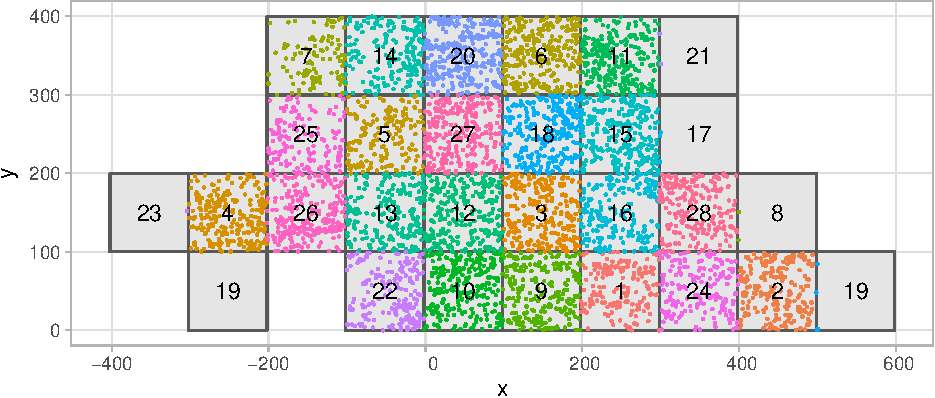
\includegraphics[width=1\linewidth]{Figures/bw-define-cv-folds-with-trees-1} 

}

\caption{Inspect blocks closely.}\label{fig:bw-define-cv-folds-with-trees}
\end{figure}

Then remove empty folds

\begin{Shaded}
\begin{Highlighting}[]
\NormalTok{growth_bw <-}\StringTok{ }\NormalTok{growth_bw }\OperatorTok
\StringTok{  }\KeywordTok{filter}\NormalTok{(}\OperatorTok{!}\NormalTok{foldID }\OperatorTok\StringTok{ }\KeywordTok{c}\NormalTok{(}\DecValTok{19}\NormalTok{, }\DecValTok{23}\NormalTok{, }\DecValTok{21}\NormalTok{, }\DecValTok{17}\NormalTok{, }\DecValTok{8}\NormalTok{, }\DecValTok{19}\NormalTok{)) }\OperatorTok
\StringTok{  }\KeywordTok{mutate}\NormalTok{(}\DataTypeTok{foldID =} \KeywordTok{factor}\NormalTok{(foldID))}
\end{Highlighting}
\end{Shaded}

Separately, we save the spatial cross-validation grid as an
\texttt{sf\_polygon} object \texttt{blocks\_bw}

\begin{Shaded}
\begin{Highlighting}[]
\NormalTok{blocks_bw <-}\StringTok{ }\NormalTok{bw_spatialBlock}\OperatorTok{$}\NormalTok{blocks }\OperatorTok
\StringTok{  }\KeywordTok{st_as_sf}\NormalTok{()}
\end{Highlighting}
\end{Shaded}

\hypertarget{scbi-1}{%
\subsubsection{SCBI}\label{scbi-1}}

First, we indicate which trees are part of the buffer. In this case
however we manually define the study region boundary based on the
subregion we defined in Section \ref{scbi-data} and create an
\texttt{sf\_polygon} object using the \texttt{sf\_polygon()} function
from the \texttt{sfheaders} package. Figure \ref{fig:scbi-define-buffer}
displays the resulting buffer trees.

\begin{Shaded}
\begin{Highlighting}[]
\NormalTok{study_region_scbi <-}\StringTok{ }\KeywordTok{tibble}\NormalTok{(}
  \DataTypeTok{x =} \KeywordTok{c}\NormalTok{(}\DecValTok{0}\NormalTok{, }\DecValTok{300}\NormalTok{, }\DecValTok{300}\NormalTok{, }\DecValTok{0}\NormalTok{, }\DecValTok{0}\NormalTok{),}
  \DataTypeTok{y =} \KeywordTok{c}\NormalTok{(}\DecValTok{300}\NormalTok{, }\DecValTok{300}\NormalTok{, }\DecValTok{600}\NormalTok{, }\DecValTok{600}\NormalTok{, }\DecValTok{300}\NormalTok{)}
\NormalTok{) }\OperatorTok
\StringTok{  }\KeywordTok{sf_polygon}\NormalTok{()}

\NormalTok{growth_scbi <-}\StringTok{ }\NormalTok{growth_scbi }\OperatorTok
\StringTok{  }\KeywordTok{add_buffer_variable}\NormalTok{(}\DataTypeTok{direction =} \StringTok{"in"}\NormalTok{, }\DataTypeTok{size =}\NormalTok{ comp_dist, }\DataTypeTok{region =}\NormalTok{ study_region_scbi)}

\KeywordTok{ggplot}\NormalTok{() }\OperatorTok{+}
\StringTok{  }\KeywordTok{geom_sf}\NormalTok{(}\DataTypeTok{data =}\NormalTok{ growth_scbi, }\KeywordTok{aes}\NormalTok{(}\DataTypeTok{col =}\NormalTok{ buffer), }\DataTypeTok{size =} \FloatTok{0.5}\NormalTok{)}
\end{Highlighting}
\end{Shaded}

\begin{figure}

{\centering 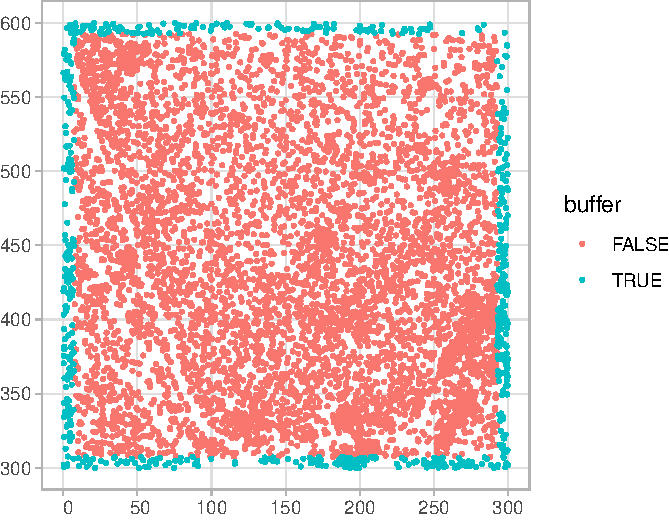
\includegraphics[width=0.5\linewidth]{Figures/scbi-define-buffer-1} 

}

\caption{Buffer region for SCBI study region.}\label{fig:scbi-define-buffer}
\end{figure}

Second, we associate each tree to spatial cross validation folds. In
this case we manually define a spatial crossvaliation grid. Figure
\ref{fig:scbi-define-cv-folds} displays the resulting cross-validation
folds along with the buffer from Figure \ref{fig:scbi-define-buffer}.

Here we manually define the spatial cross-validation grid as an
\texttt{sf\_polygon} object \texttt{scbi\_cv\_grid}

\begin{Shaded}
\begin{Highlighting}[]
\NormalTok{fold1 <-}\StringTok{ }\KeywordTok{rbind}\NormalTok{(}\KeywordTok{c}\NormalTok{(}\DecValTok{0}\NormalTok{, }\DecValTok{300}\NormalTok{), }\KeywordTok{c}\NormalTok{(}\DecValTok{150}\NormalTok{, }\DecValTok{300}\NormalTok{), }\KeywordTok{c}\NormalTok{(}\DecValTok{150}\NormalTok{, }\DecValTok{600}\NormalTok{), }\KeywordTok{c}\NormalTok{(}\DecValTok{0}\NormalTok{, }\DecValTok{600}\NormalTok{))}
\NormalTok{fold2 <-}\StringTok{ }\KeywordTok{rbind}\NormalTok{(}\KeywordTok{c}\NormalTok{(}\DecValTok{150}\NormalTok{, }\DecValTok{300}\NormalTok{), }\KeywordTok{c}\NormalTok{(}\DecValTok{300}\NormalTok{, }\DecValTok{300}\NormalTok{), }\KeywordTok{c}\NormalTok{(}\DecValTok{300}\NormalTok{, }\DecValTok{600}\NormalTok{), }\KeywordTok{c}\NormalTok{(}\DecValTok{150}\NormalTok{, }\DecValTok{600}\NormalTok{))}

\NormalTok{blocks_scbi <-}\StringTok{ }\KeywordTok{bind_rows}\NormalTok{(}
  \KeywordTok{sf_polygon}\NormalTok{(fold1),}
  \KeywordTok{sf_polygon}\NormalTok{(fold2)}
\NormalTok{) }\OperatorTok
\StringTok{  }\KeywordTok{mutate}\NormalTok{(}\DataTypeTok{folds =} \KeywordTok{c}\NormalTok{(}\DecValTok{1}\NormalTok{, }\DecValTok{2}\NormalTok{) }\OperatorTok\StringTok{ }\KeywordTok{factor}\NormalTok{())}
\end{Highlighting}
\end{Shaded}

\begin{Shaded}
\begin{Highlighting}[]
\NormalTok{SpatialBlock_scbi <-}\StringTok{ }\KeywordTok{spatialBlock}\NormalTok{(}
  \DataTypeTok{speciesData =}\NormalTok{ growth_scbi, }\DataTypeTok{k =} \DecValTok{2}\NormalTok{, }\DataTypeTok{selection =} \StringTok{"systematic"}\NormalTok{, }\DataTypeTok{blocks =}\NormalTok{ blocks_scbi,}
  \DataTypeTok{showBlocks =} \OtherTok{FALSE}\NormalTok{, }\DataTypeTok{verbose =} \OtherTok{FALSE}
\NormalTok{)}

\CommentTok{# Add foldID to each tree}
\NormalTok{growth_scbi <-}\StringTok{ }\NormalTok{growth_scbi }\OperatorTok
\StringTok{  }\KeywordTok{mutate}\NormalTok{(}\DataTypeTok{foldID =}\NormalTok{ SpatialBlock_scbi}\OperatorTok{$}\NormalTok{foldID }\OperatorTok\StringTok{ }\KeywordTok{factor}\NormalTok{())}

\KeywordTok{ggplot}\NormalTok{() }\OperatorTok{+}
\StringTok{  }\KeywordTok{geom_sf_text}\NormalTok{(}\DataTypeTok{data =}\NormalTok{ growth_scbi, }\KeywordTok{aes}\NormalTok{(}\DataTypeTok{label =}\NormalTok{ foldID, }\DataTypeTok{col =}\NormalTok{ buffer)) }\OperatorTok{+}
\StringTok{  }\KeywordTok{geom_sf}\NormalTok{(}\DataTypeTok{data =}\NormalTok{ blocks_scbi, }\DataTypeTok{fill =} \StringTok{"transparent"}\NormalTok{)}
\end{Highlighting}
\end{Shaded}

\begin{figure}

{\centering 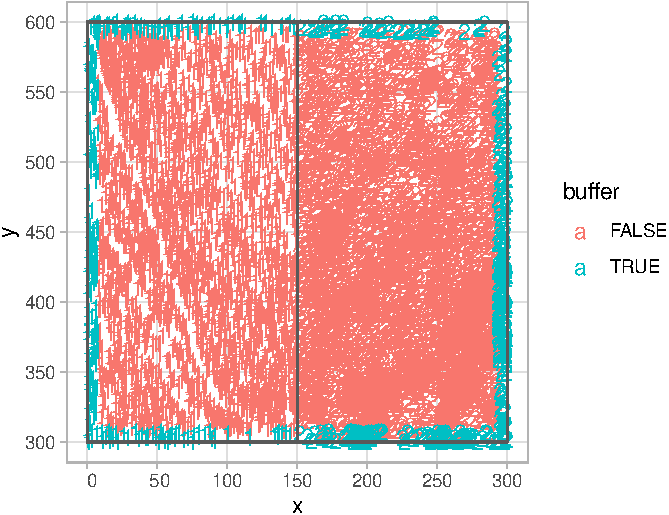
\includegraphics[width=0.5\linewidth]{Figures/scbi-define-cv-folds-1} 

}

\caption{Buffer region for SCBI study region.}\label{fig:scbi-define-cv-folds}
\end{figure}

\hypertarget{define-focal-versus-competitor-trees}{%
\subsection{Define focal versus competitor
trees}\label{define-focal-versus-competitor-trees}}

Next we define \texttt{focal\_vs\_comp} data frames which connects each
focal tree in the \texttt{growth\_df} data frames to the trees in its
competitive neighborhood range as defined by the \texttt{comp\_dist}
constant. So for example, if \texttt{growth\_df} consisted of two focal
trees with two and three neighbors with \texttt{comp\_dist}
respectively, \texttt{focal\_vs\_comp} would be a data frame of 5 rows
connecting each focal tree to it's competitors. The
\texttt{create\_focal\_vs\_comp()} function makes this connection taking
as inputs the \texttt{growth\_df} data frame; the \texttt{comp\_dist}
constant defining competitive range; \texttt{cv\_grid\_sf}, giving the
cross validation grid; and the \texttt{id} variable.

\hypertarget{big-woods-3}{%
\subsubsection{Big Woods}\label{big-woods-3}}

\begin{Shaded}
\begin{Highlighting}[]
\NormalTok{focal_vs_comp_bw <-}\StringTok{ }\NormalTok{growth_bw }\OperatorTok
\StringTok{  }\KeywordTok{create_focal_vs_comp}\NormalTok{(comp_dist, }\DataTypeTok{cv_grid_sf =}\NormalTok{ blocks_bw, }\DataTypeTok{id =} \StringTok{"treeID"}\NormalTok{)}
\end{Highlighting}
\end{Shaded}

TODO: Figure out how to show this data frame's contents.

\hypertarget{scbi-2}{%
\subsubsection{SCBI}\label{scbi-2}}

\begin{Shaded}
\begin{Highlighting}[]
\NormalTok{focal_vs_comp_scbi <-}\StringTok{ }\NormalTok{growth_scbi }\OperatorTok
\StringTok{  }\KeywordTok{create_focal_vs_comp}\NormalTok{(comp_dist, }\DataTypeTok{cv_grid_sf =}\NormalTok{ blocks_scbi, }\DataTypeTok{id =} \StringTok{"stemID"}\NormalTok{)}
\end{Highlighting}
\end{Shaded}

TODO: Figure out how to show this data frame's contents.

\hypertarget{model-fit-predict}{%
\subsection{Fit model and make predictions}\label{model-fit-predict}}

Next we fit the following linear model to the dbh of each focal tree.
Let \(i = 1, \ldots, n_j\) index all \(n_j\) trees of ``focal'' species
group \(j\); let \(j = 1, \ldots, J\) index all \(J\) focal species
groups; and let \(k = 1, \ldots, K\) index all \(K\) ``competitor''
species groups. We modeled the growth in diameter per year \(y_{ij}\)
(in centimeters per year) of the \(i^{th}\) tree of focal species group
\(j\) as a linear model \(f\) of the following covariates
\(\vec{x}_{ij}\)

\[
\newcommand{\dbh}{\text{DBH}}
\newcommand{\biomass}{\text{biomass}}
\newcommand{\BA}{\text{BA}}
y_{ij} = f(\vec{x}_{ij}) + \epsilon_{ij} = \beta_{0,j} + \beta_{\dbh,j} \cdot \dbh_{ij} + \sum_{k=1}^{K} \lambda_{jk} \cdot \BA_{ijk} + \epsilon_{ij}
\]

We estimate the model's parameters using Bayesian linear regression
implemented in the \texttt{fit\_bayesian\_model()} function. TODO:
define all parameters

For this linear model's case, there exists a closed form solution as
described here. As such, the \texttt{fit\_bayesian\_model()} function
using matrix algebra to obtain all parameter estimates, rather than
computationally expensive Monte Carlo approximations. The inputs to this
function are a \texttt{focal\_vs\_comp} data frame,
\texttt{prior\_param} a list of priors, and a boolean flag
\texttt{run\_shuffle} on whether or not to run competitor-species
identity permutations which we will demonstrate below on the Michigan
Big Woods data. This function returns the posterior means of all
parameters.

Using these posterior means, we then use the posterior predictive
distribution to obtain fitted/predicted values \(\widehat{y}\) of the
dbh for each focal tree using the \texttt{predict\_bayesian\_model()}.
These \(\widehat{y}\) can then be compared to the observed \(y\) dbh's
to compute the root mean-square error, a measure of a model's predictive
error which has the same units as the observed data \(y\).

\hypertarget{big-woods-4}{%
\subsubsection{Big Woods}\label{big-woods-4}}

For the Michigan Big Woods data we present two use cases of the model
fitting and prediction scheme. The first use case is the simplest where
we assess the fit of the model using root mean squared error. The second
use case then answers the question of whether species competitor
identity matters using permutation test.

For the first use case, we fit the linear model specified in Equation
XXX to our data frame of type \texttt{focal\_vs\_comp}. This
input/outputs of the \texttt{fit\_bayesian\_model()} function are lists
of the prior/posterior means of parameters of the linear regression
specified in XXX. Generally speaking, there are two classes of
regression parameters: \(\beta\) main effects and \(\lambda\)
competitive effects. In the upcoming Section
\ref{viz-posterior-distributions}, we will present code visualizing this
posterior distributions.

\begin{Shaded}
\begin{Highlighting}[]
\NormalTok{comp_bayes_lm_bw <-}\StringTok{ }\NormalTok{focal_vs_comp_bw }\OperatorTok
\StringTok{  }\KeywordTok{comp_bayes_lm}\NormalTok{(}\DataTypeTok{prior_param =} \OtherTok{NULL}\NormalTok{)}
\end{Highlighting}
\end{Shaded}

This output of posterior parameters for the specified competition model
are then used along with the posterior predictive distribution encoded
in \texttt{predict\_bayesian\_model()} to return predicted growths for
each individual tree. We join these predicted growths to the original
growth data frame.

\begin{Shaded}
\begin{Highlighting}[]
\NormalTok{focal_vs_comp_bw <-}\StringTok{ }\NormalTok{focal_vs_comp_bw }\OperatorTok
\StringTok{  }\KeywordTok{mutate}\NormalTok{(}\DataTypeTok{growth_hat =} \KeywordTok{predict}\NormalTok{(comp_bayes_lm_bw, focal_vs_comp_bw))}
\end{Highlighting}
\end{Shaded}

We then use the \texttt{rmse()} function from the \texttt{yardstick}
package to obtain the root mean squared error of the observed versus
fitted values of growth.

\begin{Shaded}
\begin{Highlighting}[]
\NormalTok{focal_vs_comp_bw }\OperatorTok
\StringTok{  }\KeywordTok{rmse}\NormalTok{(}\DataTypeTok{truth =}\NormalTok{ growth, }\DataTypeTok{estimate =}\NormalTok{ growth_hat) }\OperatorTok
\StringTok{  }\KeywordTok{pull}\NormalTok{(.estimate)}
\CommentTok{## [1] 0.148145}
\end{Highlighting}
\end{Shaded}

The second use case is near identical to the first, but with a small
change in the code to test whether the identity of the competitor
matters. By adding a \texttt{run\_shuffle\ =\ TRUE} argument to
\texttt{fit\_bayesian\_model()}, for each focal tree its competitor
trees' species identity will be ``shuffled'' randomly much like in a
permutation test. By shuffling these species labels we are effectively
fitting the model under a null model that competitor species identity
does not matter. If the ``shuffled'' RMSE's are consistently lower than
the unshuffled RMSE corresponding to the observed data, then we have
evidence to suggest that competitor identity matters to competitive
interactions.

\begin{Shaded}
\begin{Highlighting}[]
\NormalTok{comp_bayes_lm_bw_shuffle <-}\StringTok{ }\NormalTok{focal_vs_comp_bw }\OperatorTok
\StringTok{  }\KeywordTok{comp_bayes_lm}\NormalTok{(}\DataTypeTok{prior_param =} \OtherTok{NULL}\NormalTok{, }\DataTypeTok{run_shuffle =} \OtherTok{TRUE}\NormalTok{)}
\end{Highlighting}
\end{Shaded}

\begin{Shaded}
\begin{Highlighting}[]
\NormalTok{focal_vs_comp_bw <-}\StringTok{ }\NormalTok{focal_vs_comp_bw }\OperatorTok
\StringTok{  }\KeywordTok{mutate}\NormalTok{(}\DataTypeTok{growth_hat_shuffle =} \KeywordTok{predict}\NormalTok{(comp_bayes_lm_bw_shuffle, focal_vs_comp_bw))}
\end{Highlighting}
\end{Shaded}

\begin{Shaded}
\begin{Highlighting}[]
\NormalTok{focal_vs_comp_bw }\OperatorTok
\StringTok{  }\KeywordTok{rmse}\NormalTok{(}\DataTypeTok{truth =}\NormalTok{ growth, }\DataTypeTok{estimate =}\NormalTok{ growth_hat_shuffle) }\OperatorTok
\StringTok{  }\KeywordTok{pull}\NormalTok{(.estimate)}
\CommentTok{## [1] 0.1505383}
\end{Highlighting}
\end{Shaded}

The RMSE is fact lower for the non-shuffled version, indicative of a
better model fit. This gives support for the idea that competitor
identity does matter for competitive interactions. In
\citet{allen_permutation_2020} we run this shuffle a large number of
times to construct a full permutation distribution to show that this
difference is robust to resampling variation.

\hypertarget{scbi-3}{%
\subsubsection{SCBI}\label{scbi-3}}

In the case of the SCBI data, we once again perform the same model
fitting and computing of fitted growths as with the Big Woods data, but
this time we map the residuals of the observed minus fitted values to
look for spatial patterns.

\begin{Shaded}
\begin{Highlighting}[]
\NormalTok{comp_bayes_lm_scbi <-}\StringTok{ }\NormalTok{focal_vs_comp_scbi }\OperatorTok
\StringTok{  }\KeywordTok{comp_bayes_lm}\NormalTok{(}\DataTypeTok{prior_param =} \OtherTok{NULL}\NormalTok{)}
\end{Highlighting}
\end{Shaded}

\begin{Shaded}
\begin{Highlighting}[]
\NormalTok{focal_vs_comp_scbi <-}\StringTok{ }\NormalTok{focal_vs_comp_scbi }\OperatorTok
\StringTok{  }\KeywordTok{mutate}\NormalTok{(}\DataTypeTok{growth_hat =} \KeywordTok{predict}\NormalTok{(comp_bayes_lm_scbi, focal_vs_comp_scbi))}
\end{Highlighting}
\end{Shaded}

\begin{Shaded}
\begin{Highlighting}[]
\NormalTok{focal_vs_comp_scbi }\OperatorTok
\StringTok{  }\KeywordTok{rmse}\NormalTok{(}\DataTypeTok{truth =}\NormalTok{ growth, }\DataTypeTok{estimate =}\NormalTok{ growth_hat) }\OperatorTok
\StringTok{  }\KeywordTok{pull}\NormalTok{(.estimate)}
\CommentTok{## [1] 0.1281398}
\end{Highlighting}
\end{Shaded}

In Figures \ref{fig:scbi-model-residuals} and
\ref{fig:scbi-model-residuals-2} we present the residuals.

\begin{figure}

{\centering 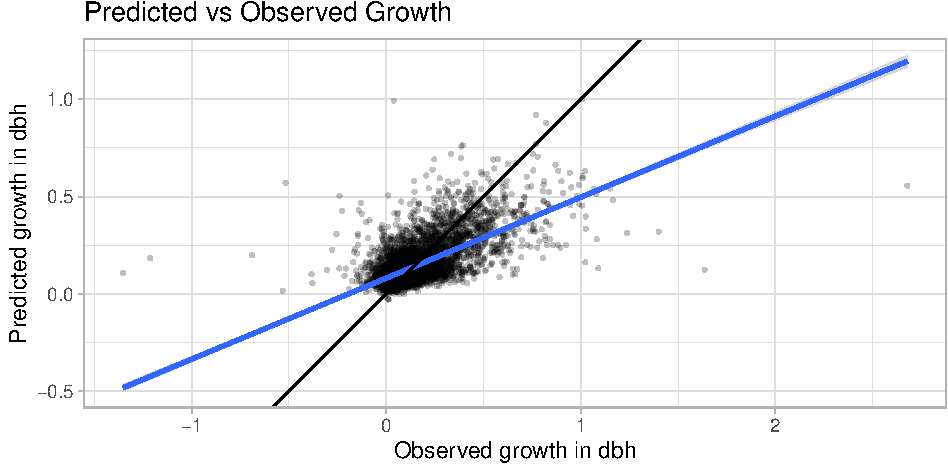
\includegraphics[width=1\linewidth]{Figures/scbi-model-residuals-1} 

}

\caption{Predicted versus observed growth.}\label{fig:scbi-model-residuals}
\end{figure}

\begin{figure}

{\centering 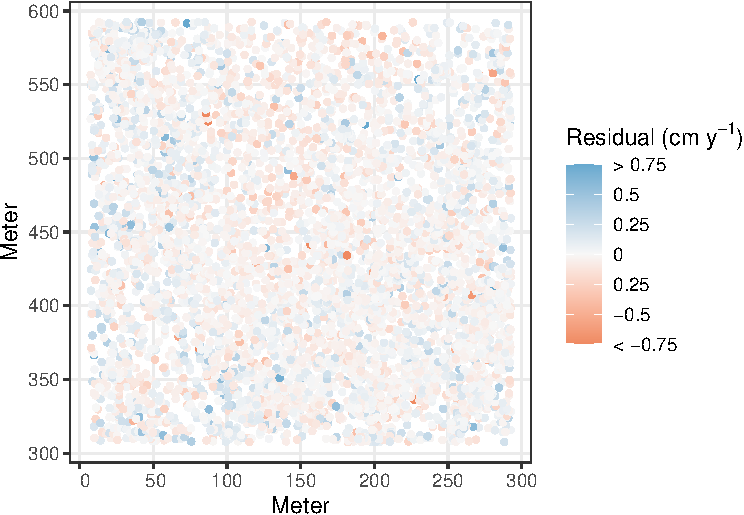
\includegraphics[width=0.8\linewidth]{Figures/scbi-model-residuals-2-1} 

}

\caption{Spatial distribution of residuals for model applied to SCBI data.}\label{fig:scbi-model-residuals-2}
\end{figure}

\hypertarget{run-spatial-cross-validation}{%
\subsection{Run spatial
cross-validation}\label{run-spatial-cross-validation}}

The model fits and predictions in Section \ref{model-fit-predict} all
suffer from a common failing: they use the same data to both fit the
model and to assess the model's performance using the RMSE. As argued by
\citet{roberts_cross-validation_2017}, this can lead to overly
optimistic assessments of model quality as the models can be overfit, in
particular in situations where spatial-autocorrelation is present. To
mitigate the effects of such overfitting, we use a spatially block
cross-validation algorithm implemented in the \texttt{run\_cv()}. This
function at its core uses the same model fitting implemented in the
\texttt{fit\_bayesian\_model()} function, however trains the model on
\(k-1\) spatial folds of the train and returns fitted values for the
test data. Recall that the spatial blocking scheme wass encoded in
Section \ref{spatial-information}.

\hypertarget{big-woods-5}{%
\subsubsection{Big Woods}\label{big-woods-5}}

Applying this spatially cross-validated model fit yields an RMSE is
higher than that when the model is fit without cross validation. In
other words, our model fits in \ref{model-fit-predict} were overly
optimistic in the model's fitting power, whereas a cross-validated
results yield an estimate that is closer to the truth. See
\citet{allen_permutation_2020} for more discussion of this.

\begin{Shaded}
\begin{Highlighting}[]
\NormalTok{focal_vs_comp_bw <-}\StringTok{ }\NormalTok{focal_vs_comp_bw }\OperatorTok
\StringTok{  }\KeywordTok{run_cv}\NormalTok{(}\DataTypeTok{comp_dist =}\NormalTok{ comp_dist, }\DataTypeTok{cv_grid =}\NormalTok{ blocks_bw)}

\NormalTok{focal_vs_comp_bw }\OperatorTok
\StringTok{  }\KeywordTok{rmse}\NormalTok{(}\DataTypeTok{truth =}\NormalTok{ growth, }\DataTypeTok{estimate =}\NormalTok{ growth_hat) }\OperatorTok
\StringTok{  }\KeywordTok{pull}\NormalTok{(.estimate)}
\CommentTok{## [1] 0.1532316}
\end{Highlighting}
\end{Shaded}

\hypertarget{scbi-4}{%
\subsubsection{SCBI}\label{scbi-4}}

Observe once again that this RMSE is much higher than that for the above
SCBI model fit without cross-validation.

\begin{Shaded}
\begin{Highlighting}[]
\NormalTok{focal_vs_comp_scbi <-}\StringTok{ }\NormalTok{focal_vs_comp_scbi }\OperatorTok
\StringTok{  }\KeywordTok{run_cv}\NormalTok{(}\DataTypeTok{comp_dist =}\NormalTok{ comp_dist, }\DataTypeTok{cv_grid =}\NormalTok{ blocks_scbi)}

\NormalTok{focal_vs_comp_scbi }\OperatorTok
\StringTok{  }\KeywordTok{rmse}\NormalTok{(}\DataTypeTok{truth =}\NormalTok{ growth, }\DataTypeTok{estimate =}\NormalTok{ growth_hat) }\OperatorTok
\StringTok{  }\KeywordTok{pull}\NormalTok{(.estimate)}
\CommentTok{## [1] 0.144608}
\end{Highlighting}
\end{Shaded}

\hypertarget{viz-posterior-distributions}{%
\subsection{Visualize posterior
distributions}\label{viz-posterior-distributions}}

Lastly, we return to the model fits from Section \ref{model-fit-predict}
and present tools to visually explore the posterior distributions of all
parameters in our model. There are two main groups of parameters to
consider. The \(\beta\) coefficients tell us about how fast each species
grows and how this depends on DBH while the full matrix of \(\lambda\)
values describe the competitive effects between pairs of species. There
is a rich literature on this matrix (cite).

DO WE NEED TO DESCRIBE MECHANICS? Because of the structure of the
\texttt{bw\_fit\_model} object we cannot simply draw these curves based
on the posterior distribution. \texttt{bw\_fit\_model()} gives the
parameters \emph{compared} to a baseline. This is not of direct
interest. So to display these parameters, as we care about them, we have
to sample from the baseline distribution and from the comparison one to
get the posterior distribution of interest.

\hypertarget{big-woods-6}{%
\subsubsection{Big Woods}\label{big-woods-6}}

Here we re-run the model fit to the Big Woods data from Section
\ref{model-fit-predict}, but this time use ``family'' as the group for
comparison which has. This makes the posterior distributions easier to
follow. Also, surprisingly, grouping by family performed just as well as
grouping by species \citet{allen_permutation_2020}. First we re-run
\texttt{create\_focal\_vs\_comp()} and \texttt{fit\_bayesian\_model()}
with no permutation shuffling with the grouping variable as family.

\begin{Shaded}
\begin{Highlighting}[]
\NormalTok{focal_vs_comp_bw <-}\StringTok{ }\NormalTok{growth_bw }\OperatorTok
\StringTok{  }\KeywordTok{mutate}\NormalTok{(}\DataTypeTok{sp =}\NormalTok{ family }\OperatorTok\StringTok{ }\KeywordTok{factor}\NormalTok{()) }\OperatorTok
\StringTok{  }\KeywordTok{create_focal_vs_comp}\NormalTok{(}\DataTypeTok{comp_dist =}\NormalTok{ comp_dist, }\DataTypeTok{cv_grid_sf =}\NormalTok{ blocks_bw, }\DataTypeTok{id =} \StringTok{"treeID"}\NormalTok{)}

\NormalTok{comp_bayes_lm_bw <-}\StringTok{ }\NormalTok{focal_vs_comp_bw }\OperatorTok
\StringTok{  }\KeywordTok{comp_bayes_lm}\NormalTok{(}\DataTypeTok{prior_param =} \OtherTok{NULL}\NormalTok{)}
\end{Highlighting}
\end{Shaded}

Now the posterior parameter outputs of \texttt{fit\_bayesian\_model()}
are passed to \texttt{plot\_bayesian\_model\_parameters()} to generate
visualizations of the posterior parameters. These visualizations are
displayed in Figure 5 of \citet{allen_permutation_2020}. For simplicity
we only plot a subset of the species families.

\begin{Shaded}
\begin{Highlighting}[]
\NormalTok{sp_to_plot <-}\StringTok{ }\KeywordTok{c}\NormalTok{(}\StringTok{"cornaceae"}\NormalTok{, }\StringTok{"fagaceae"}\NormalTok{, }\StringTok{"hamamelidaceae"}\NormalTok{, }\StringTok{"juglandaceae"}\NormalTok{, }
                 \StringTok{"lauraceae"}\NormalTok{, }\StringTok{"rosaceae"}\NormalTok{, }\StringTok{"sapindaceae"}\NormalTok{, }\StringTok{"ulmaceae"}\NormalTok{)}
\end{Highlighting}
\end{Shaded}

The output is a list with three plots stored. Figure
\ref{fig:bw-posterior-viz-beta0} The element \texttt{beta\_0} gives the
baseline growth intercept \(\beta_0\), i.e., how fast an individual of
each group grows independent of DBH).

\begin{Shaded}
\begin{Highlighting}[]
\NormalTok{plot1 <-}\StringTok{ }\KeywordTok{autoplot}\NormalTok{(comp_bayes_lm_bw, }\DataTypeTok{type =} \StringTok{"intercepts"}\NormalTok{)}
\NormalTok{plot1}
\end{Highlighting}
\end{Shaded}

\begin{figure}

{\centering \includegraphics[width=1\linewidth]{Figures/bw-posterior-viz-beta0-1} 

}

\caption{Posterior distribution of beta0.}\label{fig:bw-posterior-viz-beta0}
\end{figure}

Figure \ref{fig:bw-posterior-viz-beta-dbh} Next \texttt{beta\_dbh} gives
the slope for DBH slope \(\beta_{dbh,i}\) for each group.

\begin{Shaded}
\begin{Highlighting}[]
\NormalTok{plot2 <-}\StringTok{ }\KeywordTok{autoplot}\NormalTok{(comp_bayes_lm_bw, }\DataTypeTok{type =} \StringTok{"dbh_slopes"}\NormalTok{)}
\NormalTok{plot2}
\end{Highlighting}
\end{Shaded}

\begin{figure}

{\centering \includegraphics[width=1\linewidth]{Figures/bw-posterior-viz-beta-dbh-1} 

}

\caption{Posterior distribution of betadbh.}\label{fig:bw-posterior-viz-beta-dbh}
\end{figure}

Finally Figure \ref{fig:bw-posterior-viz-lambda} \texttt{lambda} gives
the competition coefficients \(\lambda\).

\begin{Shaded}
\begin{Highlighting}[]
\NormalTok{plot3 <-}\StringTok{ }\KeywordTok{autoplot}\NormalTok{(comp_bayes_lm_bw, }\DataTypeTok{type =} \StringTok{"competition"}\NormalTok{)}
\NormalTok{plot3}
\end{Highlighting}
\end{Shaded}

\begin{figure}

{\centering \includegraphics[width=1\linewidth]{Figures/bw-posterior-viz-lambda-1} 

}

\caption{Posterior distribution of lambda's for Big Woods.}\label{fig:bw-posterior-viz-lambda}
\end{figure}

\hypertarget{scbi-5}{%
\subsubsection{SCBI}\label{scbi-5}}

We revisit the posterior parameters for the SCBI from Section
\{model-fit-predict\}, but this time only focus on the \(\lambda\)
competition coefficients.

\begin{Shaded}
\begin{Highlighting}[]
\NormalTok{sp_to_plot <-}\StringTok{ }\KeywordTok{c}\NormalTok{(}\StringTok{"quru"}\NormalTok{, }\StringTok{"litu"}\NormalTok{, }\StringTok{"cagl"}\NormalTok{, }\StringTok{"cato"}\NormalTok{)}
\end{Highlighting}
\end{Shaded}

\begin{Shaded}
\begin{Highlighting}[]
\NormalTok{plot3 <-}\StringTok{ }\KeywordTok{autoplot}\NormalTok{(comp_bayes_lm_bw, }\DataTypeTok{type =} \StringTok{"competition"}\NormalTok{)}
\NormalTok{plot3}
\end{Highlighting}
\end{Shaded}

\begin{figure}

{\centering \includegraphics[width=1\linewidth]{Figures/scbi-posterior-viz-lambda-1} 

}

\caption{Posterior distribution of lambda's for SCBI.}\label{fig:scbi-posterior-viz-lambda}
\end{figure}

Add explanation here.

HEY BERT PICK IT UP HERE

\hypertarget{discussion}{%
\section{Discussion}\label{discussion}}

\hypertarget{acknowledgments}{%
\section{Acknowledgments}\label{acknowledgments}}

\bibliographystyle{agsm}
\bibliography{paper.bib}

\end{document}
